% !TeX document-id = {c74a84f4-c0b2-4978-a479-47211c753752}
% !BIB TS-program = biber

\documentclass[twocolumn]{article}

\usepackage{algorithm}
\usepackage{algpseudocode}
\usepackage{amsfonts}
\usepackage{amsmath}
\usepackage{biblatex}
\usepackage{caption}
\usepackage{dirtytalk}
\usepackage{hyperref}
\usepackage{mathtools}
\usepackage{multicol}
\usepackage{placeins}
\usepackage{siunitx}
\usepackage{subcaption}
\usepackage{tikz}
\usepackage{url}
\usepackage{xypic}

\title{Skip Ratchet \\[1ex] \large A Hierarchical Hash System}
\author{Brooklyn Zelenka \\ \href{https://fission.codes}{Fission Codes} \\ \href{mailto:brooklyn@fission.codes}{brooklyn@fission.codes} }
\addbibresource{spiral-ratchet.bib}
\date{\today\\v1.0.1}

\begin{document}
    \maketitle
    
%    \begin{multicols}{2}
    
   	\begin{abstract}\
   		Hash chains are a simple way to generate pseudorandom key material. However, they are inefficient in many situations, including when used as logical clocks, or for synchronizing the heads of a forward secret stream. This paper presents the ``skip ratchet'', a novel symmetric key derivation function that can be efficiently incremented by arbitrary intervals.
   	\end{abstract}

   	\section{Introduction}
   	
	Hash algorithms provide a way to generate pseudorandom data from an input that is impractical to reverse. Many applications iteratively hash a value (``ratcheting'' \cite{pond}) for pre-computation resistance, forward secrecy (FS), one-time schemes (e.g. S/KEY \cite{rfc1760}), deterministically generating unique names, key derivation functions (KDFs), digital payment schemes \cite{multidimensional}, and so on.
	
	This paper introduces the ``skip ratchet'', a hierarchical and iterative hashing system suitable for symmetric key derivation, and capable of efficiently making large leaps in hash count while preserving forward secrecy in a passive setting.

    \section{Motivation}
    
    The intersection of private data and location-independent access control in open protocols is only beginning to be explored. Decentralization and trust minimization are increasingly important, but admit to many unsolved problems including how to secure changing data in an unknown and unstable topology. Not knowing the number or attributes of peers implies the use of passive security methods based directly on data.
    
    An increasing number of applications in open decentralized networks have no fixed topology, and require zero-interaction key agreement on a large number of files, the ability to share a single file (and no others), a range of files, or elements from a point in time onwards (but not prior versions). As such, there is also a need to keep the historical information of the internal state secret from even those with current access.
    
    One approach for securing history is to use a simple ratchet function, iteratively hashing on each update to produce the next state (a "hash chain"). This works well if the number of changes to synchronize is small, but $\mathcal{O}(n)$ ratchet steps is prohibitive as the difference grows. It allows a malicious participant to force others to a large amount of work in order to access the latest update.
    
    The skip ratchet presented here improves the situation. A skip ratchet is able to synchronize in sublinear time, supports efficient arbitrary access in the forward direction, maintains backwards secrecy of its internal state, and does not leak metadata such as the number of updates or participants. Further, jump size and granularity are configurable.
    
    \section{Numeral Intuition}
    
    The problem of how to efficiently calculate the $n^{\text{th}}$ step of a ratchet in less than $n$ steps is structurally similar to how we efficiently represent large numbers. There are many systems for doing so. The two most common are tally marks (unary) and positional numeral systems. The skip ratchet uses both of these concepts.
    
	\subsection{Unary Hashing}

	Hash chains are structurally very similar to unary counting systems.\footnote{Two examples are tally marks and Peano numbers \cite{peano-wikipedia}.} Unary is very concrete: the symbol count is equivalent to the number being represented. Replacing the successor function with a hash function $h$, one may represent unary counting with hashes.\footnote{By convention, this paper will use $I$, $J$, and $K$ as independent fixed initial values, $x$ as an arbitrary variable, and $h$ for hashing} Importantly, this does not make reference to a concrete ``zero'' value; merely an interval from the input $x$.
	
	While this method is very straightforward, it is not time efficient. A unary digit is included in the skip ratchet for forward security reasons. However, the remaining digits are more efficient.
	
    \begin{figure}[h]
		\centering
		
		\begin{flalign}
			Peano(3) & \Rightarrow S(S(S(0))) \nonumber \\
			h_{chain}(3)  & \Rightarrow h(h(h(I))) \equiv h^{3}(I) \nonumber 
		\end{flalign}
	
		\caption{Peano Number $\leftrightarrow$ Hash Chain}
		\label{fig:peano-hash-equiv}
	\end{figure}
    
    \subsection{Positional Hashing}
    
    A major advantage of positional numerals is the ability to express large jumps with minimal effort. In positional systems (such as the familiar binary, decimal, and hexadecimal) each position corresponds to some factor for the numeral at that position.\footnote{While most systems use fixed-base exponential factors, there exist systems where there is no common relationship between positions.}
    
    \begin{figure}[h]
       	\centering
        $246_{16}$ = 2$\times{16^{2}}$ + 4$\times{16^{1}}$ + 6$\times{16^{0}}$ = $582_{10}$
     \caption{Componentized Hexadecimal}
    \end{figure}
    
    Just as positional numerals combine multiple numbers to represent a single sum, a KDF state can have multiple components that are combined to create a single symmetric key.\footnote{Different directions of this core idea include hash calendars \cite{distributed-hash-calendar}, and multidimensional hash chains (MDHC) \cite{multidimensional}}
    
    \begin{figure}[h]
       	\begin{flalign}
       		h_{10}(x+0)   & \Rightarrow I \nonumber \\
       		h_{10}(x+11)  & \Rightarrow \langle h(J), h(I) \rangle \nonumber \\
       		h_{10}(x+582) & \Rightarrow \langle h^{5}(K), h^{8}(J), h^{2}(I) \rangle \nonumber 
       	\end{flalign}
       	
       	\caption{Compound Hash State}
       	\label{fig:compound-hash}
    \end{figure}
    
    Unlike a positional number system used in arithmetic, a KDF ``forgets'' its internal state, combining elements and flattening its structure. There are many methods of combination, including further hashing; this paper will use bitwise \textsf{XOR} (Figure \ref{fig:compound-kdf}).
    
	\begin{figure}[h]
		\begin{flalign}
			h_{pos10, \oplus}(0)   & \Rightarrow I \nonumber \\
			h_{pos10, \oplus}(11)  & \Rightarrow h(J) \oplus h(I) \nonumber \\
			h_{pos10, \oplus}(582) & \Rightarrow h^{5}(K) \oplus h^{8}(J) \oplus h^{2}(I) \nonumber 
		\end{flalign}
	
		\caption{Compound Hash Key Derivation}
		\label{fig:compound-kdf}
	\end{figure}
    
    \section{Bounding}
    
    Unlike numeral systems useful for arithmetic, the skip ratchet's internal state is composed of a fixed number of ``digits''. This limits the jumps to fixed intervals, with a maximum jump interval. While it is possible to create variants that deterministically generate increasingly large digits as needed, but this would leak data about the range of the counter. Being computationally indistinguishable is desirable in many use cases, such as for securing updatable documents in an public network.
    
    While advancing the ratchet by arbitrary intervals is possible, the jump operation is not the same as adding arbitrary integers. Incrementing all but the lowest digit cascades down to the lower values, ``zeroing'' them out. Therefore, arbitrary jumps require a carry (Algorithm \ref{alg:jump}). This is structurally similar to deterministic skip lists \cite{deterministic-skip-lists} (Figure \ref{fig:skip-list}), but with each step pointing to a monotonically increasing value, rather than previous ones.\footnote{While the analogy to fingered DAGs such as skip lists in the name is apt, the skip ratchet is distinct from other DAG-structured hash constructions like the Merkle tree \cite{merkle-tree} or hash calendar \cite{distributed-hash-calendar}. A skip ratchet does not aggregate digests into a signature, but rather counts by iteratively hashing the same value repeatedly, in tiers.} \\
 
	\begin{figure*}[h]
		\centering
		
		$\xymatrix{
			  Nil
			& A \ar[l]
			& B \ar[l] , \ar@/^1pc/[ll]
			& C \ar[l]
			& D \ar[l] , \ar@/^1pc/[ll] , \ar@/_2pc/[llll]
			& E \ar[l]
			& F \ar[l] , \ar@/^1pc/[ll]
			& G \ar[l]
			& H \ar[l] , \ar@/^1pc/[ll] , \ar@/_2pc/[llll]
		}$
	
		\caption{Deterministic Skip List}
		\label{fig:skip-list}
	\end{figure*}

	\begin{figure*}[h]
		\centering
		
		$\xymatrix{
		    \underset{000_{2}}{\left[ { \begin{array}{cc} L \\ M  \\ S \end{array} } \right]}
				\ar[r]^{+1}
				\ar@/_3pc/[rr]_{skip_{M}}
				\ar@/^7pc/[rrrr]^{skip_{L}}
    	 & \underset{001_{2}}{\left[ { \begin{array}{cc} L \\ M  \\ h(S) \end{array} } \right]}
	      		\ar[r]^{+1}
	      		\ar@/^4.75pc/[rrr]^{skip_{L}}
	     & \underset{010_{2}}{\left[ { \begin{array}{cc} L \\ h(M)  \\ S' \end{array} } \right]}
	      		\ar[r]^{+1}
	      		\ar@/_3pc/[rr]_{skip_{M}}
	      		\ar@/^3pc/[rr]^{skip_{L}}
    	 & \underset{011_{2}}{\left[ { \begin{array}{cc} L \\ h(M)  \\ h(S') \end{array} } \right]}
	      		\ar[r]^{+1}
	     & \underset{100_{2}}{\left[ { \begin{array}{cc} h(L) \\ M'  \\ S'' \end{array} } \right]}
		}$

		\caption{Simplified Skip Ratchet}
		\label{fig:compound-ratchet}
	\end{figure*}

	Each digit is given a label and maximum value for all but the largest, which acts as a linear ``spine''. This largest element is analogous to an unbounded unary digit. The remaining elements are arranged positionally, and are bounded by their numerical base. Since the unary digit is a hard limit on the number of digits, it conceals information about the range of numbers that the current internal state represents. Any range within a fixed larger value is called an ``epoch'' (e.g. ``the 300s epoch'' or ``the $h^{42}(x)$ epoch'').\footnote{The term ``epoch'' is used here in the generic or Ethereum\cite{ethereum-yellowpaper} sense, and is a slightly different from some other ratchet constructions such as the Double Ratchet\cite{double-ratchet-modularization}.}
	
	By geometric analogy, the possible steps in this construction are similar to moving along a spiral: one component returns to its initial value, but the other dimension is always moving forward. Following a spiral in single steps is smooth, but leaps are possible by jumping to adjacent rings (Figure \ref{fig:spiral-metaphor}). Unlike the repeating numerals found in most counting systems, the skip ratchet never repeats a value despite the counter being kept to a limited number of elements. We call this the ``spiral property.''
	
	\begin{figure}[h]
		\centering
		
		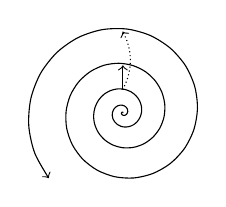
\begin{tikzpicture}
			\draw [->, domain=0:29, variable=\t, smooth, samples=100]
			plot ({\t r}: {0.0015 * \t * \t});
			\draw [->] (0, 0.3) -- (0, 0.6);
			\draw [->, style=densely dotted, rotate=-30] (-0.15, 0.250) arc (0:60:21pt);
		\end{tikzpicture}
		
		\caption{Spiral With Leaps}
		\label{fig:spiral-metaphor}
	\end{figure}
	
	\section{Skip Ratchet}
	
	\subsection{Internal State}
	
	The skip ratchet's state is built from a unary digit $U$, a fixed number $n$ of positional digits, and their base $b$. The positional digits are bounded by the base, and so must track a natural number count. The unary digit explicitly does not track its count.
	
	\begin{figure*}[h]
		\centering
		
		$S : \langle \langle Count_{0}, Value_{0} \rangle, \langle Count_{1}, Value_{1} \rangle \ldots \langle Count_{n-1}, Value_{n-1} \rangle, U\rangle_{b}$
		
		\caption{Skip Ratchet Counter State}
		\label{fig:counter}
	\end{figure*}

	Note that Figure \ref{fig:counter} is given as little-endian. The order of the state does not strictly matter, but it is convenient to associate the index of the state with the exponent for the base that the position represents.
	
	\subsection{Initialization}
	
	A skip ratchet is deterministically derived from a hash function $h$, a numeric base $b$, a positional digit count $n$, a function $k$ to derive a key the state, and an initialization vector $IV$. We distinguish between configurations by referring to their $\langle n, b, h, k \rangle$ triple, such as $\langle 3, 256, \textsf{SHA}3, \oplus \rangle$ skip ratchet.\footnote{This also implies that a $\langle 1, b, h, k \rangle$ skip ratchet would merely be a hash chain.}

	\begin{figure}[h]
		\centering
	
		$(\langle n, b, h, k \rangle, IV) \rightarrow S$
	
		\caption{Seed Generation}
		\label{fig:config}
	\end{figure}
	
	To prevent leaking the iteration count, all of the positional values in the seed state are immediately incremented by a random value. This randomized origin is treated as the ratchet's starting state. Given the backward secrecy constraint, only relative values may be used unless this initial value is known.
	
	Each positional value is generated from the \emph{binary complement ($\sim$) of the preimage} of its larger neighbour, in a recursive cascade starting with the unary digit (Algorithm \ref{alg:setup}). This protects the information needed to derive the current state, and thus prevents leaking all of the values in that range.
		
	\begin{algorithm*}
		\begin{algorithmic}[1]
			\Require $\langle n, b, k \rangle \in \mathbb{N}_{1}\times{\mathbb{N}_{1}\times{\mathbb{N}_{1}}}$
			\State $seed \overset{\$}{\gets} \lbrace 0, 1 \rbrace^{k}$
			\State $pos   \coloneqq []$
			\State $unary \coloneqq hash(seed)$
			\For{$i \gets (n - 1) \ldots 0$} \Comment{Descending to associate index with degree}
				\State $\delta \overset{\$}{\gets} 0\ldots{b - 1}$
				\State $seed \coloneqq hash(\sim{seed})$ \Comment{Secretly derive from the larger value}
				\State $pos[i].count \coloneqq \delta$
				\State $pos[i].value \coloneqq hash^{\delta + 1}(seed)$
			\EndFor
			\\
			\Return{$b, unary, pos$}
		\end{algorithmic}
	
		\caption{Skip Ratchet Initialization}
		\label{alg:setup}
	\end{algorithm*}

	The number of digits is configurable. These should be chosen to a balance jump control (the number of intervals that can be skipped by), and step-function performance. If the number of digits is large, increment on the unary element or higher digits will have require multiple hash operations in each zero cascade.
	
	In practice, $\langle 3, 256, \textsf{SHA}3, \oplus \rangle$ and $\langle 3, 256, \textsf{BLAKE}3, \oplus \rangle$ skip ratchets have performed well. The maximum leap is $256^{2}$, so the state $i + 256^{3}$ is (approximately) the same amount of work as $i + 256$. Given the small constant factor of hardware-accelerated hashing and the monotonicity of a ratchet, relatively large bases are often viable.

	\subsection{Basic Operations}
	
	Basic operations on the skip ratchet follow from the rules set out during initialization. It can be incremented sequentially, or leap to the next ``zero'' of any digit. Any interval can be efficiently found by combining increments and skips (Figure \ref{fig:sr-ops}).
	
	It is sometimes helpful to distinguish between a small and large skip, and so the terms ``skip'' and ``leap'' may be used for this purpose, despite them functioning identically but on different positions. The term ``increment'' (or ``inc'') is only used for the special case of the smallest movement (by one).
	
	\begin{figure*}[h]
		\centering
		
		$\xymatrix{
			IV \ar[r]^<<<<<{inc} 
				& *+[F]{State_{0}}
					\ar[d]|\oplus
					\ar[r]^{inc}
					\ar@/^1.5pc/[rr]^{skip}
					\ar@{.>}@/^5pc/[rrrr]^{leap}
				& *+[F]{State_{1}}
					\ar[d]|\oplus
					\ar[r]^{inc}
					\ar@{.>}@/^3pc/[rrr]^{leap}
				& *+[F]{State_{2}} 
					\ar[d]|\oplus
					\ar[r]^{inc}
					\ar@/^1.5pc/[rr]^{skip}
				& *+[F]{State_{3}}
					\ar[d]|\oplus
					\ar[r]^{inc}
				& *+[F]{State_{4}}
					\ar[d]|\oplus
					\ar[r]^{inc}
				& \cdots
			\\
				& \text{Key}_{0}
				& \text{Key}_{1}
				& \text{Key}_{2}
				& \text{Key}_{3}
				& \text{Key}_{4}
		}$
		
		\caption{Binary Skip Ratchet Operations}
		\label{fig:sr-ops}
	\end{figure*}

	Being a ratchet, it can never be ``unwound'' (there is no inverse or subtractive analogue). Access to earlier keys requires knowing an even earlier state, and moving forward to the desired state from there. This is important for break-in resistance and backwards secrecy (e.g sharing a document from a point in time but no earlier).

	\subsubsection{Key Derivation}

	Generating output key material (OKM) from the ratchet state can be done in a myriad of ways. This paper will use the bitwise \textsf{XOR} function, as it is straightforward and efficient.

	\begin{algorithm*}
		\caption{Generating a Key}
		\label{alg:toKey}

		\begin{algorithmic}[1]
			\Function{toKey}{ratchet}
				\State $sum \coloneqq ratchet.unary$
				\For{$digit \in ratchet.pos$}
					\State $sum \coloneqq acc \oplus digit.value$
				\EndFor
				\State $\textbf{return}\ sum$
			\EndFunction
		\end{algorithmic}
	\end{algorithm*}
	
	\subsubsection{Increment}
	
	As with positional numerals, when a digit reaches its maximum, the next larger digit is incremented, and all lower digits are zeroed out. The zero cascade works similarly for skip ratchets, but never repeats a value (i.e. the \hyperref[{spiral-metaphor}]{spiral property}). As during initialization, the initialization, each zero is derived from the preimage of the higher digit.
	
	The special case of incrementing by one is the simplest way to demonstrate this (Algorithm \ref{alg:inc}). It functions by checking the lowest digit's counter, and if it's saturated, mark a carry and move to the next digit and recurse, bounded by the unary digit. Any carried digits are then re-zeroed by the preimage of their larger neighbour.
	
	\begin{algorithm*}
		\caption{Incrementing a Skip Ratchet}
		\label{alg:inc}

		\begin{algorithmic}[1]
			\Function{inc}{$ratchet$}
				\State $\{base, unary, pos\} \gets ratchet$
				\State $seed \coloneqq unary$
				\State $counter \coloneqq length(pos)$
				\\
				\For{$i \gets 0 \ldots length(pos) - 1$}
					\State $\{count, value\} \gets pos[i]$
					\If{$count \overset{?}{<} base - 1$} \Comment{Position not saturated}
						\State $seed \coloneqq value$
						\State $counter \coloneqq i$
						\State $ratchet.pos[i].count \coloneqq count + 1$ \State $ratchet.pos[i].value \coloneqq hash(value)\}$
						\State \textbf{break}
					\EndIf
				\EndFor
				\\
				\If{$counter\overset{?}{=} length(pos)$} \Comment{All positional values were saturated}
					\State $ratchet.unary \coloneqq hash(unary)$
				\EndIf
				\\
				\If{$counter \overset{?}{>} 0$}
					\For{$j \gets (counter - 1) \ldots 0$} \Comment{N.B. Descending}
						\State $seed' \coloneqq pos[j].value$
						\State $ratchet[pos][j].count \coloneqq 0$
						\State $ratchet[pos][j].value \coloneqq hash(\sim{seed})$
						\State $seed \coloneqq seed'$
					\EndFor
				\EndIf
				\\
				\State $ratchet$
				\EndFunction
		\end{algorithmic}
	\end{algorithm*}

	\subsubsection{Arbitrary Jumps}

	Jumps by an arbitrary interval require a little more calculation (Algorithm \ref{alg:jump}). The interval $\delta$ is componentized, and each digit incremented in ascending order. Every positional digit has an upper bound, so any remainder saved for the final step, where any zeroed digits are incremented to match the final count. Arbitrary jumps run in $\mathcal{O}(\log_{b} \delta)$ when $\delta < b^{b(n+1)}$ (the normal operating interval that the skip ratchet is tuned for). As the unary hash chain dominates as $\delta$ becomes very large, the complexity becomes $\mathcal{O}(\frac{\delta}{b^{n}})$.

	\begin{algorithm*}[b]
		\caption{Skip Ratchet Arbitrary Jump}
		\label{alg:jump}
		
		\begin{algorithmic}[1]
			\Function{jump}{$ratchet, amount$}
				\State $\{base, unary, pos\} \gets ratchet$
				\State $remaining \coloneqq amount$
				\State $seed \coloneqq unary$
				\State $carry \coloneqq []$
				\State $n \coloneqq length(pos)$
				\\
				\For{$i \gets 0 \ldots n - 1$}
					\If{$remaining \overset{?}{=} 0$}
						\State \textbf{break}
					\EndIf
					\\
					\State $component_{i} \coloneqq remaining\mod{base^{i}}$
					\State $remaining \coloneqq remaining - component_{i}$
					\State $\delta_{i} \coloneqq \frac{component}{base^{i}}$ \Comment{No remainder because ascending in steps}
					\\
					\State $\{count, value\} \gets pos[i]$
					\State $headroom \coloneqq base - count - 1$
					\\
					\If{$\delta_{i} \overset{?}{>} headroom$}
						\State $carry[i] \coloneqq steps - headroom$
					\Else
						\State $ratchet.pos[i].count \coloneqq count + \delta_{i}$
						\If{$remaining \overset{?}{=} 0$}
							\State $seed \coloneqq hash^{\delta_{i} - 	1}(value)$
							\State $ratchet.pos[i].value \coloneqq hash(seed)$
						\Else
							\State $carry[i] \coloneqq 0$
						\EndIf
					\EndIf
				\EndFor
				\\
				\If{$remaining \overset{?}{>} 0$}
					\State $component_{u} \coloneqq remaining \mod{base^{n}}$
					\State $\delta_{u} \coloneqq \frac{component_{u}}{base^{n}}$
					\State $ratchet.unary \coloneqq hash^{\delta_{u}}(unary)$
				\EndIf
				\\
				\For{$j \gets (length(carry) - 1) \ldots 0$} \Comment{N.B. Descending}
					\State $seed \coloneqq hash^{carry[j] - 1}(\sim{seed})$
					\State $ratchet.pos[j].value \coloneqq hash(seed)$
				\EndFor
				\\
				\State $\textbf{return}\ ratchet$
			\EndFunction
		\end{algorithmic}
	\end{algorithm*}

	\section{Security}
	
	There is no inbuilt way to revoke this access once the key is compromised. Updates rely on forward secrecy for protection, and key rotation in the case where a breach becomes known. Algorithms like the Double Ratchet\cite{double-ratchet} have post-compromise security in a two-party semi-trusted setup, where there key is automatically rotated as a matter of course.
		
	The skip ratchet has two security domains: its external key generation, and its internal state. The internal state is itself based on hierarchical hash chains to assure forward secrecy, even for those that have been given access to the KDF's internal state. Not only is the previous state not calculable, other metadata such as the number of steps is also hidden, even when the internal state is known.
	
	\subsection{Interval Bounding}
	
	The skip ratchet's internal state permits bounding derivation to a fixed range in a decentralized system. This is accomplished by only sharing a few of the lower positions, and only sharing the rest of te state as a flattened hash.
	
	Revealing one OKM provides access to the cleartexts encrypted with that key (e.g. a single version of one file). Providing the \textsf{XOR} of the unary digit and a nonzero number of positional elements gives (post-compromise) access to the remaining number of updates in that epoch. Access to the entire internal state grants access from a point onwards, including potentially the initial state. As such, the number of elements in the internals state must be at least $n+2$ to provide if intended for use in this setting, where $n$ is the number of levels that are desired to be exposed.
	
	For example, in a $\langle 4, 256, \textsf{SHA}3, \oplus \rangle$ skip ratchet, sharing $\langle S, M, L \oplus U \rangle$ allows the recipient to move freely in the ``medium'' jump range, up to $i + 256^{3} - 1$. Keys can still be fully generated thanks to \textsf{XOR}'s associativity, but the recipient will need to ask for the next $L' \oplus U$ to continue.
	
	\subsection{Post-Compromise Security}
	
	The skip ratchet trades off general post-compromise self-healing (of the unary digit) for permissionless key agreement between an unbounded and growable set of peers. If the secured communications are between exactly two parties, the Double Ratchet is typically a better choice due to its post-compromise security. Such a model could be adapted to use a skip ratchet for decentralized key agreement over time. In essence, this involves distributing a freshly initialized skip ratchet to a list of trusted peers on every $i$ steps \cite{decentralized-key-agreement}, or any other method of rotating the unary digit.
	
	\section{Conclusion}
	
	This paper has presented the skip ratchet, an algorithm for decentralized key agreement on streams of encrypted data with unbounded and changing participants. Arbitrary forward search in the expected operating range can be performed in $\mathcal{O}(\log_{b} \delta)$ time, backwards access is impossible without the earlier internal state, and total counts can never be inferred from the internal state.
    
    \section{Acknowledgements}
    
    The skip ratchet algorithm was developed at \href{https://fission.codes}{Fission Codes} to support work on the \href{https://github.com/fission-suite/webnative}{WebNative File System (WNFS)}. Many thanks to the Fission Codes team for providing the support and freedom to develop this algorithm.
    
    Thanks to \href{https://github.com/matheus23/}{Philipp Krüger} at Fission Codes for  feedback on the design, for writing the bulk of the TypeScript implementation\cite{ts-wnfs-ratchet}, and for his patience as various parts of the algorithm were tweaked while that code was already in-flight.
    
    Many thanks to \href{https://github.com/QuinnWilton}{Quinn Wilton} at Fission Codes for her feedback on various drafts of this paper, research into the broader literature, and suggestions on intended audience.
    
    Thanks to \href{https://github.com/b5/}{Brendan O'Brien} at \href{https://qri.io/}{Qri} for the {Go implementation}\cite{go-wnfs-ratchet}, and for many discussions on the best way to explain the concept.
    
    Thanks to \href{https://github.com/dholms}{Daniel Holmgren} at \href{https://blueskyweb.xyz}{Bluesky} for his feedback on early versions of this algorithm.
    
    Thanks to \href{https://github.com/jbenet/}{Juan Benet} at \href{https://protocol.ai/}{Protocol Labs} for encouraging me to write a fuller description of the skip ratchet than what was available in the WebNative online documentation.

    \printbibliography[title={References}]
\end{document}
